\documentclass[a4paper, landscape,border=0.4cm]{standalone}

\usepackage{tikz}
\usetikzlibrary{arrows.meta, positioning}

\pagestyle{empty}

\begin{document}

\resizebox{\textwidth}{!}{
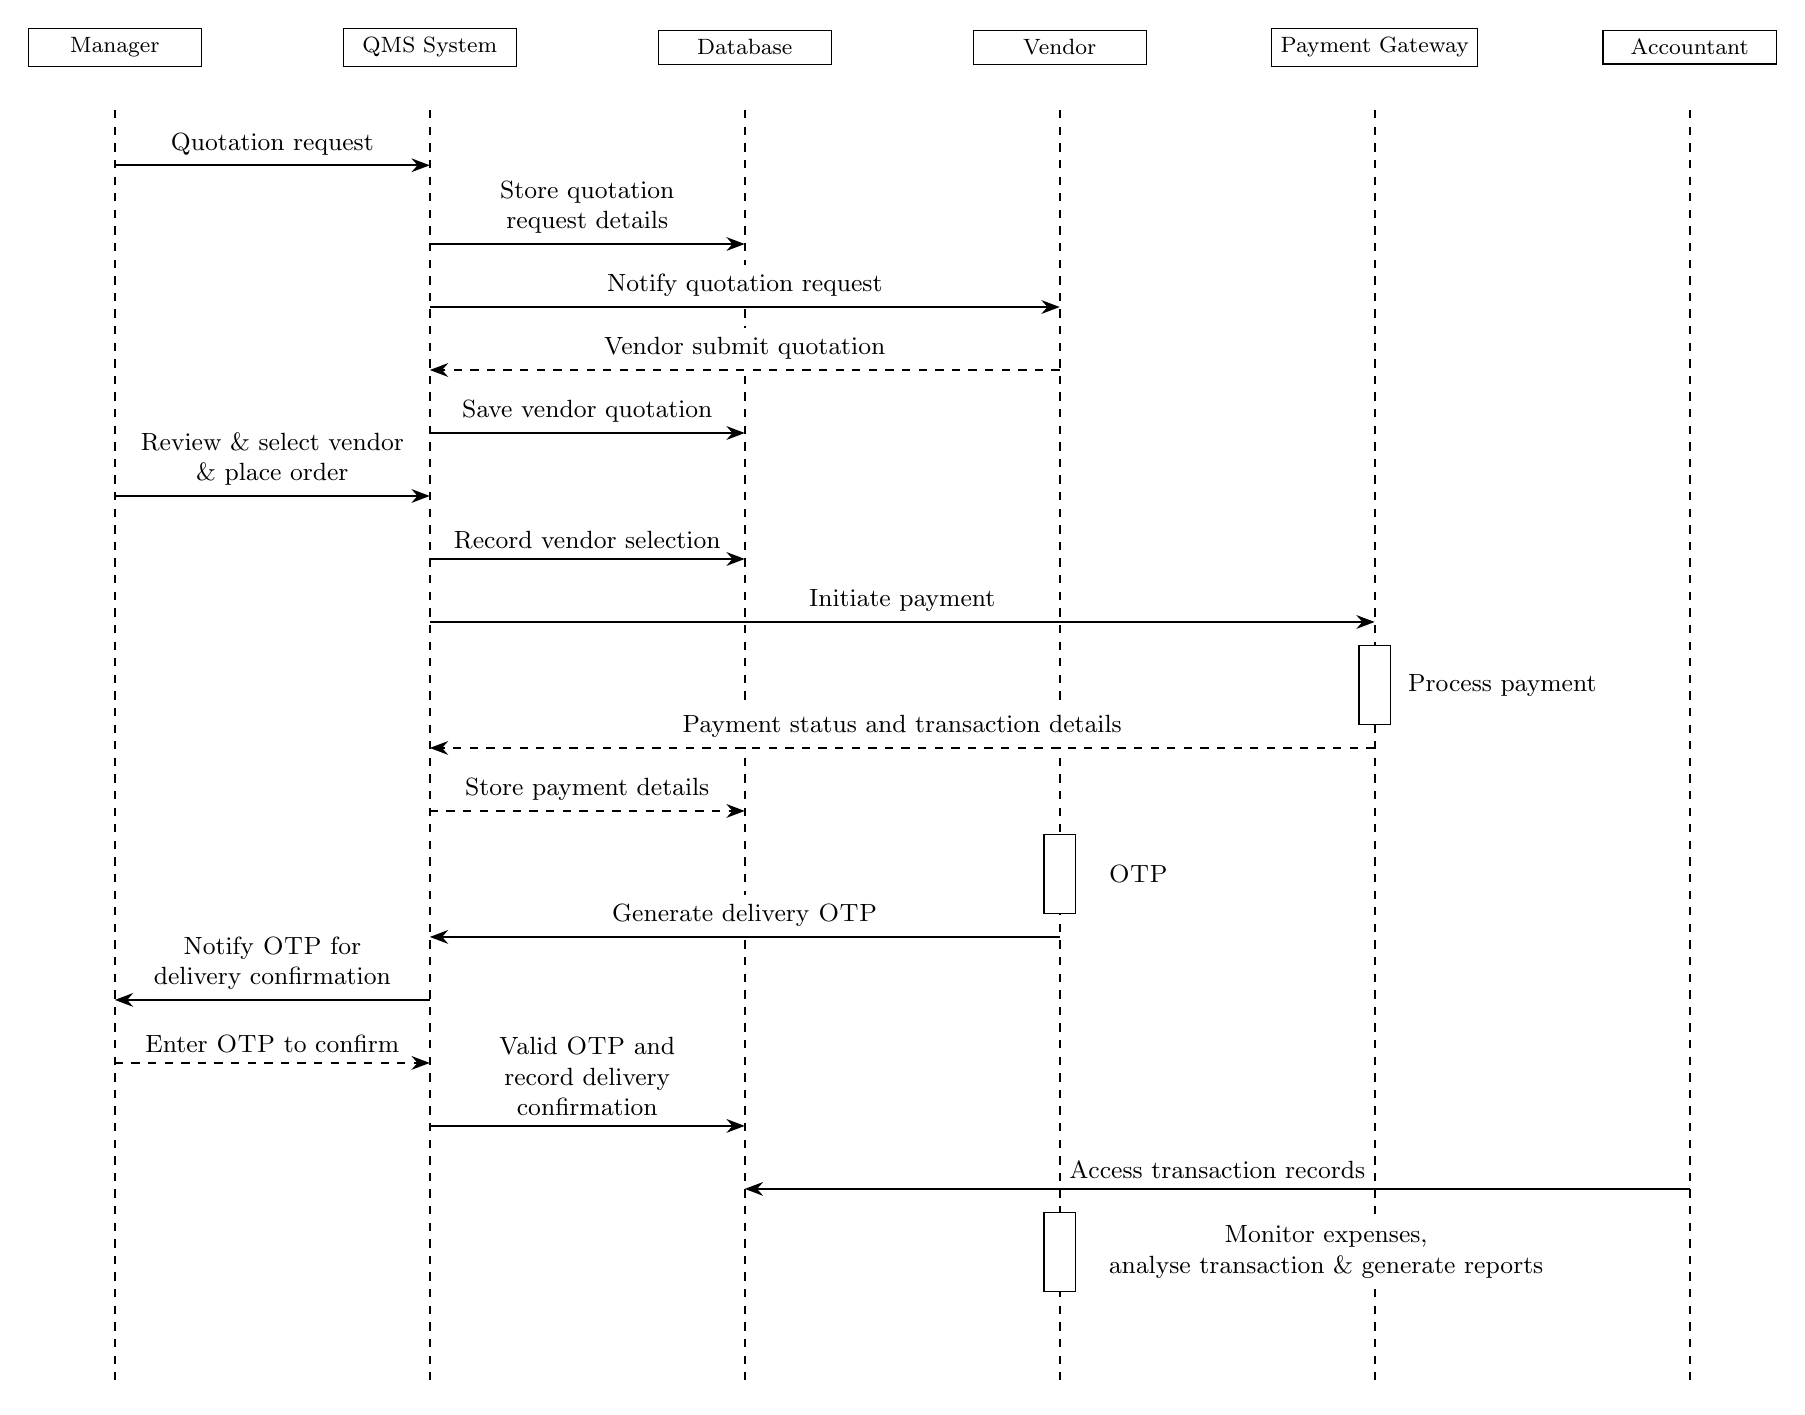
\begin{tikzpicture}[
    >=Stealth,
    lifeline/.style={draw, thick, dashed},
    message/.style={->, thick},
    return/.style={->, dashed, thick},
    activation/.style={draw, rectangle, fill=white, minimum width=0.4cm},
    font=\footnotesize
]

%-------------------------------------------------
% Participants
%-------------------------------------------------
\node[draw, rectangle, minimum width=2.2cm] (manager)    at (0,0)  {Manager};
\node[draw, rectangle, minimum width=2.2cm] (qms)        at (4,0)  {QMS System};
\node[draw, rectangle, minimum width=2.2cm] (db)         at (8,0)  {Database};
\node[draw, rectangle, minimum width=2.2cm] (vendor)     at (12,0) {Vendor};
\node[draw, rectangle, minimum width=2.2cm] (payment)    at (16,0) {Payment Gateway};
\node[draw, rectangle, minimum width=2.2cm] (accountant) at (20,0) {Accountant};

%-------------------------------------------------
% Lifelines
%-------------------------------------------------
\foreach \x in {0,4,8,12,16,20}
    \draw[lifeline] (\x,-0.8) -- (\x,-17);

%-------------------------------------------------
% Messages
%-------------------------------------------------
\draw[message] (0,-1.5) -- node[above] {\small Quotation request} (4,-1.5);

\draw[message] (4,-2.5) -- node[above, sloped,fill=white,align=center, font=\small] {Store quotation\\ request details} (8,-2.5);

\draw[message] (4,-3.3) -- node[above, sloped ,fill=white] {\small Notify quotation request} (12,-3.3);

\draw[return]  (12,-4.1)  -- node[above, sloped ,fill=white] {\small Vendor submit quotation} (4,-4.1);

\draw[message] (4,-4.9) -- node[above, sloped] {\small Save vendor quotation} (8,-4.9);

\draw[message] (0,-5.7) -- node[above, align=center, font=\small]
{Review \& select vendor\\ \& place order} (4,-5.7);

\draw[message] (4,-6.5) -- node[above, sloped] { \small Record vendor selection} (8,-6.5);

\draw[message] (4,-7.3) -- node[above, sloped] {\small Initiate payment} (16,-7.3);

%-------------------------------------------------
% Payment Processing
%-------------------------------------------------
\node[activation, minimum height=1cm] at (16,-8.1) {};
\node[right] at (16.3,-8.1) {\small  Process payment};

\draw[return] (16,-8.9) -- node[above, sloped,fill=white] {\small Payment status and transaction details } (4,-8.9);

\draw[return] (4,-9.7) -- node[above, sloped] {\small Store payment details  } (8,-9.7);

%-------------------------------------------------
% Delivery & OTP
%-------------------------------------------------

\node[activation, minimum height=1cm] at (12,-10.5) {};
\node[right] at (12.5,-10.5) {\small  \textsc{OTP}};


\draw[message] (12,-11.3) -- node[above, sloped,fill=white] {\small Generate delivery \textsc{OTP}} (4,-11.3);

%-------------------------------------------------
% Transaction Records
%-------------------------------------------------
\draw[message] (4,-12.1) -- node[above, sloped,fill=white,align=center , font =\small ] { Notify \textsc{OTP} for\\ delivery confirmation} (0,-12.1);

\draw[return] (0,-12.9) -- node[above, sloped] {\small Enter \textsc{OTP} to confirm } (4,-12.9);

\draw[message] (4,-13.7) -- node[above, sloped,fill=white,align=center,font=\small] { Valid \textsc{OTP} and\\ record delivery\\ confirmation} (8,-13.7);


\draw[message] (20,-14.5) -- node[above, sloped] {\small Access transaction records} (8,-14.5);





%---------------------------------------------------------
% Monitor transaction and expenses
%---------------------------------------------------------

\node[activation, minimum height=1cm] at (12,-15.3) {};
\node[right, align=center, font=\small ,fill=white] at (12.5,-15.3) { Monitor expenses, \\ analyse transaction \& generate reports};



\end{tikzpicture}}

\end{document}
